\section{Auswahl des Algorithmus}
\label{sec:Auswahl}
Test

\section{Implementierung in Python}

Nachdem in Kapitel \ref{sec:Auswahl} evaluiert wurde welcher Algorithmus für unsere Problematik am besten angewendet werden kann wurde die Implementierung des \glqq Bees Algorithms\grqq{} in der Programmiersprache Python programmiert.\\

Zu Beginn des Programmes musste die Karte mit den dazugehörigen Hindernissen initialisiert werden. Die Karte wurde in Form eines 2D-Koordinatensystems umgesetzt (siehe Abbildung \ref{fig:map_init}).

\begin{figure}[H]
    \begin{tabular}{@{}r@{}} 
        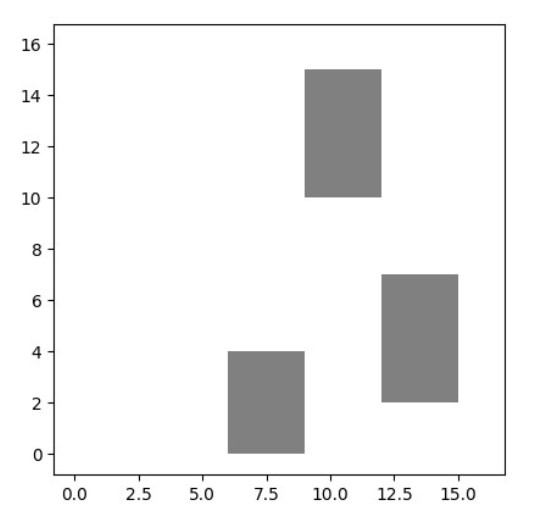
\includegraphics[width=0.5\textwidth, height=0.31\textheight, center]{map_init.jpg}
    \end{tabular}
    \caption{Initialisierte Karte mit Hindernissen\\}   
    \label{fig:map_init}
\end{figure}

